\documentclass{article}

\usepackage{scribe}

\setseriestitle{Probabilistic Machine Learning and Inference}
\setscribecode{4}
\setauthname{Gurpreet Singh}
\setinstrname{Piyush Rai}
\setheaddate{December 2, 2017}
\settitle{Hyper-Parameter Estimation using MLE-II}

\begin{document}
\makeheader

In the previous scribes, we have discussed how to estimate paramters for probabilistic models, and looked at parameter estimation for the coin-toss example as well as the regression problem. In this scribe, we will look at estimating the hyperparameters for Bayesian Regression, using the MLE-II approach.

\begin{ssection}[1]{Learning Hyperparameters}

	Let us reconsider the Bayesian Linear Regression model.

	\begin{figure}[h!]
		\centering
		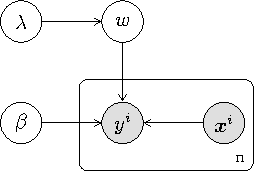
\includegraphics{includes/scribe03/bayesian-regression-model.pdf}
		\caption{Plate Notation of a Bayesian Linear Regression Model}
		\label{fig:bayes-reg-model}
	\end{figure}

	As discussed earlier, we estimate the hyperparameters using methods like Cross-Validation, however we wish to probabilitically estimate a good value for the hyperparameters. There are various methods to do this, such as

	\begin{enumerate}[label=(\roman*)]
		\item Doing point estimation of hyperparameters and learning full posterior for the parameters (MLE-II)
		\item Using general inference methods such as MCMC and Variational Bayes (Discussed in later scribes)
	\end{enumerate}

	Before we move on to learning these methods, we must first understand why we need them. Let us try a simple probabilistic approach to estimating hyperparameters (determining the full posterior). \br

	Let us first take a look at the form of the prior for the hyperparameters and the parameters (all can be considered as the parameters of the model) $\prob{\vw, \beta, \lambda}$. \br

	From the plate notation, we can say that $\beta$ and $\lambda$ are independent of other parameters, whereas $\vw$ is dependent on $\lambda$ (which makes intuitive sense as well since $\lambda$ is the precision value for the assumed gaussian that explains the distribution of $\vw$). Therefore,

	\begin{align*}
		\prob{\vw, \beta, \lambda}	\eq	\prob{\vw \pipe \lambda} \cdot \prob{\beta} \cdot \prob{\lambda}
	\end{align*}

	Now, let us try to compute the posterior ---
	\begin{align*}
		\prob{\vw, \beta, \lambda \pipe \cX, \cY}	\eq	\frac{\prob{\cY \pipe \cX, \vw, \beta, \lambda} \prob{\vw, \beta, \lambda}}{\prob{\cY \pipe \cX}}
	\end{align*}

	where
	\begin{equation}
		\prob{\cY \pipe \cX}	\eq	\int_{\vw, \beta, \lambda}	\prob{\prob{\cY \pipe \cX, \vw, \beta}} \prob{\vw, \beta, \lambda}
		\label{eq:hyper-pos}
	\end{equation}

	It can be shown that the above term is intractable. Therefore, we cannot perform Bayesian Inference on this directly. This is the reason we require different approaches to predicting the hyperparameters.

	\begin{exercise}
		Prove that the integral in Equation \ref{eq:hyper-pos} is indeed intractable.
	\end{exercise}

	\note{The approaches to estimate hyperparamters are not just limited to hyperparameters, but can also be extended for multi-parameter models}

\end{ssection}

\begin{ssection}[2]{Learning Hyperparameters}

	As mentioned in the previous section, we have the prior over $\vw, \beta, \lambda$ with the form
	\begin{equation}
		\prob{\vw, \beta, \lambda}	\eq	\prob{\vw \pipe \lambda} \cdot \prob{\beta} \cdot \prob{\lambda}
	\end{equation}

	We can also write the posterior (using Bayes Rule) as
	\begin{equation}
		\prob{\vw, \beta, \lambda \pipe \cX, \cY}	\eq	\prob{\vw \pipe \cX, \cY, \beta, \lambda} \cdot \prob{\beta, \lambda}
		\label{eq:pos-bayes}
	\end{equation}

	Now, we already know how to compute $\prob{\vw \pipe X, \vy, \beta, \lambda}$ if $\beta$ and $\lambda$ are known. However, computing $\prob{\beta, \lambda \pipe X, \vY}$ is intractable.
	\begin{align*}
		\prob{\beta, \lambda \pipe X, \vY}	\eq	\frac{\prob{\vy \pipe X, \beta, \lambda} \cdot \prob{\beta} \cdot \prob{\lambda}}{\prob{\vy \pipe X}}
	\end{align*}

	From the arguments in the discussion in \hyperlink{sec:1}{Section 1}, we know that this quantity is intractable, therfore, we need a work-around for this. \br

	A possible solution is (as already stated) take only the point estimate of $\beta$ and $\lambda$. Therfore, we only need to find an estimate of $\beta$ and $\lambda$ and plug that into the posterior for simple Bayesian Linear Regression (discussed in the previous scribe) \ie assume $\alpha$ and $\beta$ to be known. \br
	\begin{equation}
		\prob{\vw \pipe \vy, X, \wbeta, \wlambda}	\eq	\ND{\vw \pipe \vmu, \Sigma}
		\label{eq:pos-w}
	\end{equation}

	where
	\begin{align*}
		\Sigma	&\eq	\para{\wlambda \vI + \wbeta X \tr{X}}^{-1} \\
		\vmu	&\eq	\Sigma \para{\wbeta \sum_{i \in \brac{n}} y^i \vx^i}
	\end{align*}

	Therefore, we now find the point estimate of $\beta$ and $\lambda$
	\begin{align*}
		\wbeta, \wlambda	\eq	\argmax{\beta, \lambda} \prob{\beta, \lambda \pipe X, \vy}
	\end{align*}

	Note that this is MAP estimation. Therefore, we need to assume some prior on $\beta$ and $\lambda$. However, we simply assume that the priors on $\beta$ and $\lambda$ are uniform and therefore uninformative. Thus, the MAP estimation boils down to MLE estimation.
	\begin{equation}
		\wbeta, \wlambda	\eq	\argmax{\beta, \lambda} \prob{\vy \pipe X, \beta, \lambda}
		\label{eq:hyper-params}
	\end{equation}

	\begin{exercise}
		Prove that if the prior is a uniform distribution, then MAP estimate is equal to the MLE estimate.
	\end{exercise}

	\begin{remark}
		We can also do MAP estimation on $\beta$ and $\lambda$, if we assume some informative prior for them. The method could be called MAP-II
	\end{remark}

	At this point, it may seem like we are done with the estimation of the hyperparameters. However, we are missing a point. The RHS in Equation \ref{eq:hyper-params} does not have a closed form. This is evident from the following equations.
	\begin{align*}
		\prob{\vy \pipe X, \beta, \lambda}	\eq	\int_{\vw} \prob{\vy \pipe X, \vw, \beta} \cdot \prob{\vw \pipe \lambda}\ d\vw 
	\end{align*}

	We can integrate this, using properties of Gaussian Distributions, to get the following term, the intermediate steps for which are left as an exercise.
	\begin{equation}
		\prob{\vy \pipe X, \beta, \lambda}	\eq \ND{\vy \pipe \vzero, \beta^{-1} \vI + \lambda^{-1} X \tr{X}}
		\label{eq:hyper-mle}
	\end{equation}

	Now MLE solution of this is generally not in closed form, hence, we require an alternate tecnique, known as Alternating Minimization, discussed in the next section.

\end{ssection}

\begin{ssection}{Alternating Optimization}

	Suppose we already have an estimate of $\beta$ and $\lambda$. Then we know we can easily compute $\prob{\vw \pipe X, \vy, \wbeta, \wlambda}$. Also, if we have this probability, then we can easily perform MLE estimation on the term shown in Equation \ref{eq:hyper-mle}. \br

	The above suggests that we can have have an alternating approach to solving for the optimal $\beta$ and $\lambda$ and at the same time computing the posterior $\vw \pipe \vy, X$ \et{i.e.} assume some $\alpha^0$ and $\beta^0$, compute posterior in Equation \ref{eq:pos-w} and then solve for Equation \ref{eq:hyper-mle} iteratively. We give the algorithm for the alternating optimization below \br

	\begin{algo}[0.8\textwidth]{h!}{Alternating Optimization for MLE-II}

		\begin{enumerate}
			\item Initialize $\set{\wbeta}^0$ and $\set{\wlambda}^0$
			\item Repeat until convergence for t = 1, 2 $\dots$

				\begin{enumerate}
					\item Estimate the posterior over $\set{\vw}^t$ as
						\begin{align*}
							\prob{\set{\vw}^t \pipe \vy, X, \set{\wbeta}^{t-1}, \set{\wlambda}^{t-1}}	\eq	\ND{\set{\vw}^t \pipe \vmu, \Sigma}
						\end{align*}

						where $\vmu$ and $\Sigma$ are as defined in Equation \ref{eq:pos-w} \br
					\item Estimate $\wlambda^t$ and $\wbeta^t$ as
						\begin{align*}
							\set{\wlambda}^t	&\eq	\frac{\gamma}{\tr{\vmu} \vmu} \\
							\set{\wbeta}^t	&\eq	\frac{N - \gamma}{\sum_{i \in \brac{n}} \para{y^i - \tr{\vmu} \vx^i}^2}
						\end{align*}

						where $\gamma$ is a function of the eigenvalues of $\Sigma$
				\end{enumerate}
		\end{enumerate}

	\end{algo}

	Note that we do not discuss the intricacies of the algorithm or even the exact form of the algorithm, however the general idea of Alternating Optimization should be clear from this example.

	\begin{remark}
		The optimization function in Equation \ref{eq:pos-w} is a convex function, and hence, we can expect that function to always converge. Therefore, we say that Alternating Optimization for this example will always converge to a minima (local or global)
	\end{remark}

\end{ssection}<++>

\end{document}
